201~200~\documentclass[10pt]{article}
\usepackage[margin=0.9in]{geometry}
\usepackage{booktabs}
\usepackage{array}
\usepackage{xcolor}
\usepackage{colortbl}
\usepackage{tikz}
\usetikzlibrary{positioning,arrows.meta,fit,backgrounds}
\usepackage[hidelinks]{hyperref}
\usepackage{enumitem}
\setlist{nosep,leftmargin=1.4em}

\definecolor{mask}{HTML}{1F6FEB}
\definecolor{box}{HTML}{D33A4B}
\definecolor{phone}{HTML}{2EA043}
\definecolor{ink}{HTML}{1B2733}

\renewcommand{\arraystretch}{1.15}
\setlength{\parindent}{0pt}
\setlength{\parskip}{5pt}

\title{\vspace{-1.2cm}\textbf{IRIS: A Closed-Loop Face-Worn Sleep Apnea Screener\\with Integrated Positional Haptic Therapy}}
\author{\normalsize Design Brief --- Biomedical Engineering}
\date{\vspace{-0.4cm}}

\begin{document}
\maketitle
\vspace{-0.8cm}

%==================================================================
\section*{1\quad System Overview}
IRIS combines two head-worn nodes. A \textbf{sleep mask} (Seeed XIAO ESP32-S3) screens for
obstructive sleep apnea (OSA) from physiologic signals and serves a live phone dashboard.
A \textbf{haptic node} (Seeed XIAO ESP32-C6) tracks head/body orientation and delivers
positional therapy. The mask is the network hub; the phone holds all session history.

\begin{center}
\small
\begin{tabular}{@{}>{\raggedright\arraybackslash}p{3.5cm} >{\raggedright\arraybackslash}p{4.2cm} >{\raggedright\arraybackslash}p{6.0cm}@{}}
\toprule
\textbf{Sensor / Actuator} & \textbf{Node} & \textbf{Role} \\
\midrule
MAX30102 reflectance oximeter & Mask (ESP32-S3) & SpO\textsubscript{2} $\rightarrow$ desaturation index (ODI); heart rate \\
NTC thermistor (nasal airflow) & Mask (ESP32-S3) & Breath cycle; airflow cessation $\rightarrow$ apnea \\
MAX9814 microphone & Mask (ESP32-S3) & Snore index; post-apnea arousal gasp \\
MPU-6050 IMU & Haptic (ESP32-C6) & Head/body position $\rightarrow$ supine detection \\
DRV2605L + ERM motors & Haptic (ESP32-C6) & Vibrotactile positional cue \\
\bottomrule
\end{tabular}
\end{center}

%==================================================================
\section*{2\quad Base Apnea Detection}
\textbf{Primary --- Oxygen Desaturation Index (ODI).} A desaturation event is an SpO\textsubscript{2}
drop $\geq 3\%$ from a rolling baseline lasting $> 10$\,s; ODI is events per hour~\cite{odi-def}.
ODI is the validated home-screening surrogate for the lab-measured apnea--hypopnea index (AHI):
reported correlation coefficients commonly exceed $r = 0.94$~\cite{odi-corr}, and home overnight
oximetry detects OSA (AHI\,$\geq$\,5) with $\approx$\,93\% sensitivity and $\approx$\,92\%
specificity~\cite{oximetry-home}. Severity bands mirror AHI: \textbf{5--15 mild, 15--30 moderate,
$\geq$30 severe}~\cite{odi-def}.

\textbf{Corroboration --- airflow.} A thermistor airflow gap $\geq 10$\,s flags an apnea candidate;
candidates paired with a desaturation within $\sim$20\,s are scored as high-confidence events.

\textbf{Context --- sound.} A loud microphone event immediately following an airflow gap marks the
arousal/gasp that terminates an obstructive event; cumulative snore-seconds per hour give a snore index.

%==================================================================
\section*{3\quad Coupling to the Vibration Box}
The haptic node reads the IMU continuously and detects the supine position. When supine persists
beyond a threshold ($T \approx 10$--$30$\,s), the DRV2605L drives the ERM motors with
\textbf{escalating intensity}, stopping the instant a lateral position is detected --- mirroring
validated forehead/neck devices~\cite{forehead-rct,positional-pilot}. The base behavior is fully
\textbf{autonomous} (no network). Optionally, the mask may send an apnea-triggered command to the box
over the shared link, closing the detect$\rightarrow$therapy loop.

\textbf{Why position.} In $\approx$56--75\% of OSA, events are position-dependent~\cite{pt-meta}. A
meta-analysis of vibrotactile positional therapy reported a \textbf{54\% reduction in AHI} and an
\textbf{84\% reduction in supine sleep time}~\cite{pt-meta}. A forehead-worn RCT lowered AHI from
\textbf{30.6 to 20.4 events/h}~\cite{forehead-rct}; a forehead pilot cut median AHI by
\textbf{31.6\%} and raised minimum overnight SaO\textsubscript{2} from \textbf{84.3\% to
88.3\%}~\cite{positional-pilot}.

%==================================================================
\section*{4\quad Competitive Comparison}
No shipping single face-worn product both \emph{screens} via oximetry \emph{and} \emph{delivers}
positional therapy --- the two functions are split across separate products. That integration is our edge.

\begin{center}
\small
\begin{tabular}{@{}>{\raggedright\arraybackslash}p{3.3cm} >{\raggedright\arraybackslash}p{2.3cm} cc >{\raggedright\arraybackslash}p{3.6cm}@{}}
\toprule
\textbf{Device} & \textbf{Form factor} & \textbf{Detects apnea} & \textbf{Pos. therapy} & \textbf{Integration} \\
\midrule
Somnibel~\cite{forehead-rct} & Forehead & --- (position only) & Yes & Therapy-only \\
Somfit~\cite{somfit} & Forehead & Yes (PAT + ox.) & --- & Detection-only \\
Night Shift~\cite{nightshift} & Neck / chest & Snore (+ separate oximeter) & Yes & Two devices \\
NightBalance & Chest & --- (position only) & Yes & Therapy-only \\
\rowcolor{box!12}\textbf{IRIS (ours)} & \textbf{Face mask + head} & \textbf{Yes (SpO\textsubscript{2}/ODI, airflow, snore)} & \textbf{Yes} & \textbf{Closed-loop, single system} \\
\bottomrule
\end{tabular}
\end{center}

%==================================================================
\section*{5\quad System Architecture}
\begin{center}
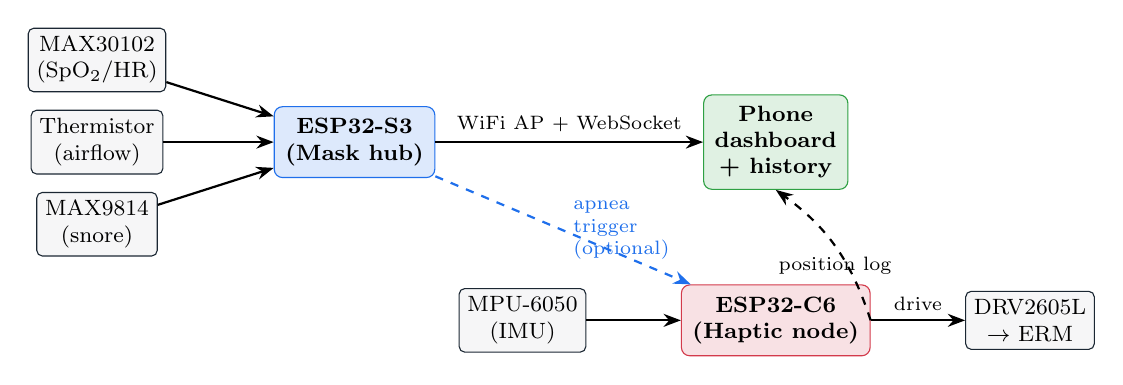
\begin{tikzpicture}[
	  font=\footnotesize,
	    >={Stealth[length=2.2mm]},
	      sensor/.style={draw=ink, rounded corners=2pt, fill=ink!4, align=center, inner sep=3pt, minimum height=7mm},
	        mcu/.style={draw, rounded corners=3pt, align=center, inner sep=4pt, minimum height=9mm, font=\footnotesize\bfseries},
	          link/.style={->, thick}
	          ]
	          % Mask sensors
	          \node[sensor] (ox)  {MAX30102\\(SpO$_2$/HR)};
	          \node[sensor, below=2.2mm of ox] (th) {Thermistor\\(airflow)};
	          \node[sensor, below=2.2mm of th] (mic){MAX9814\\(snore)};
	          % Mask MCU
	          \node[mcu, fill=mask!15, draw=mask, right=14mm of th] (s3) {ESP32-S3\\(Mask hub)};
	          % Phone
	          \node[mcu, fill=phone!15, draw=phone, right=34mm of s3] (ph) {Phone\\dashboard\\+ history};
	          % Haptic node
	          \node[mcu, fill=box!15, draw=box, below=12mm of ph] (c6) {ESP32-C6\\(Haptic node)};
	          \node[sensor, left=12mm of c6] (imu) {MPU-6050\\(IMU)};
	          \node[sensor, right=12mm of c6] (drv) {DRV2605L\\$\rightarrow$ ERM};

	          % edges
	          \draw[link] (ox)  -- (s3);
	          \draw[link] (th)  -- (s3);
	          \draw[link] (mic) -- (s3);
	          \draw[link] (s3) -- node[above,font=\scriptsize]{WiFi AP + WebSocket} (ph);
	          \draw[link] (imu) -- (c6);
	          \draw[link] (c6) -- node[above,font=\scriptsize]{drive} (drv);
	          \draw[link, dashed, mask] (s3) -- node[right,font=\scriptsize, align=left]{apnea\\trigger\\(optional)} (c6);
	          \draw[link, dashed] (c6.east) to[bend right=18] node[below,font=\scriptsize]{position log} (ph.south);
	          \end{tikzpicture}
	          \end{center}
	          \vspace{-2mm}
	          {\footnotesize Solid = wired sensor/actuator and primary data path. Dashed = optional wireless coupling.
	          The haptic node runs supine detection \& therapy independently of the network.}

	          %==================================================================
	          \begin{thebibliography}{9}
	          \footnotesize
	          \bibitem{odi-def} ``Oxygen desaturation index as an alternative parameter in screening patients with severe obstructive sleep apnea,'' \textit{[journal/authors to verify]}, NCBI PMC8889990.
	          \bibitem{odi-corr} ``Oxygen Desaturation Index (ODI): correlation with AHI ($r>0.94$),'' clinical reference summary, 2026.
	          \bibitem{oximetry-home} ``Contribution of pulse oximetry in relation to respiratory flow events in a home-based approach to diagnosing OSA,'' NCBI PMC8157782.
	          \bibitem{odi-psg} ``Correlation between oxygen desaturation index measured by overnight oximetry and AHI measured by polysomnography,'' NCBI PMC11576076.
	          \bibitem{pt-meta} ``Efficacy of new-generation positional therapy devices for positional OSA: a systematic review and meta-analysis,'' \textit{J. Clin. Sleep Med.}, 2017, doi:10.5664/jcsm.6622.
	          \bibitem{forehead-rct} ``New forehead device in positional obstructive sleep apnoea: a randomised clinical trial,'' \textit{Thorax}, 2021, PMID 33888576.
	          \bibitem{positional-pilot} ``A new postural device for the treatment of positional obstructive sleep apnea: a pilot study,'' \textit{Respir. Med.}, 2019, doi:10.1016/j.rmed.2019.02.011.
	          \bibitem{somfit} ``Evaluating Somfit's pulse arterial tonometry for detection of obstructive sleep apnoea,'' NCBI PMC11971089.
	          \bibitem{nightshift} Advanced Brain Monitoring, ``Night Shift Sleep Positioner,'' product \& validation literature (Levendowski \textit{et al.}, \textit{J. Clin. Sleep Med.}, 2014).
	          \end{thebibliography}
	          \vspace{-2mm}
	          {\scriptsize\itshape Note: reference author/volume fields are drawn from source metadata --- verify against the primary PDFs before final submission. Not a medical device; detection thresholds are screening heuristics.}

	          \end{document}
]
